%%%%%%%%%%%%%%%%%%%%%%%%%%%%%%%%%%%%%%%%%%%%%%%%%%%%%%%%%%%%%%%%%%%%%%%%%%%%%%%%%%
\begin{frame}[fragile]\frametitle{}

\begin{center}
{\Large Chunking}
\end{center}
\end{frame}

%%%%%%%%%%%%%%%%%%%%%%%%%%%%%%%%%%%%%%%%%%%%%%%%%%%%%%%%%%%%%%%%%%%%%%%%%%%%%%%%%%
\begin{frame}[fragile]
\begin{itemize}
\item chunk parsing:
  \begin{itemize}
    \item efficient and robust approach to parsing natural language
    \item a popular alternative to the full parsing
  \end{itemize}
\item chunks:
  \begin{itemize}
  \item non-overlapping regions of text
  \item contain a head word (e.g. noun)
  \item adjacent modifiers and function words
  \end{itemize}
\item motivations:
  \begin{itemize}
  \item extract information
  \item ignore information
  \end{itemize}
\end{itemize}
\end{frame}

%%%%%%%%%%%%%%%%%%%%%%%%%%%%%%%%%%%%%%%%%%%%%%%%%%%%%%%%%%
\begin{frame}[fragile]
  \frametitle{Extracting Information: Coreference Annotation}
\begin{center}
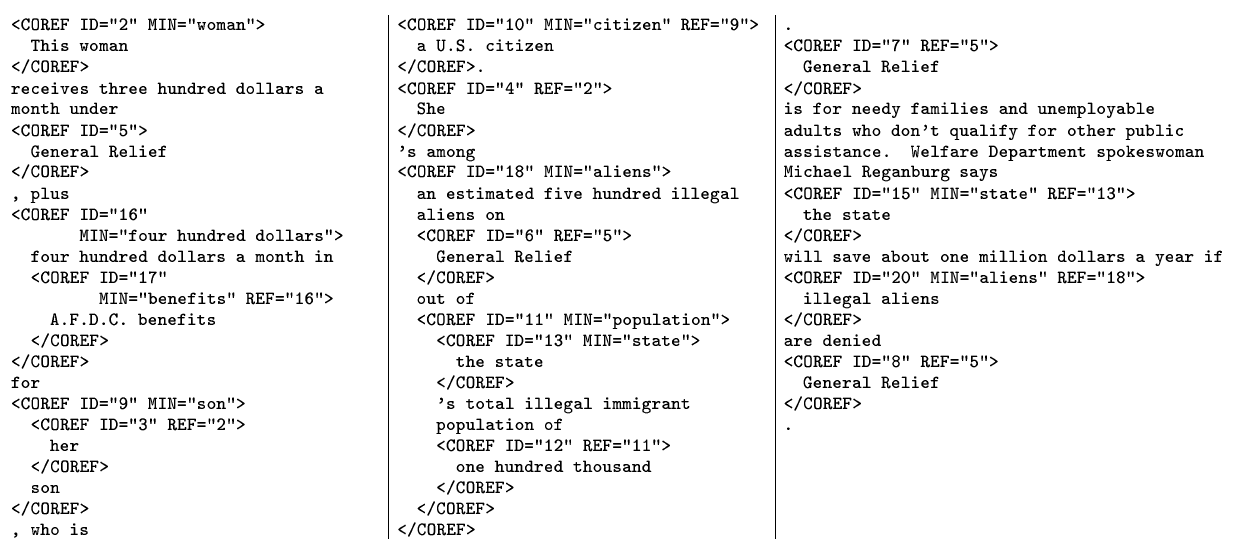
\includegraphics[width=\linewidth,keepaspectratio]{chunk-coref}
\end{center}
\end{frame}

%%%%%%%%%%%%%%%%%%%%%%%%%%%%%%%%%%%%%%%%%%%%%%%%%%%%%%%%%%
\begin{frame}[fragile]
  \frametitle{Extracting Information: Message Understanding}
\begin{center}
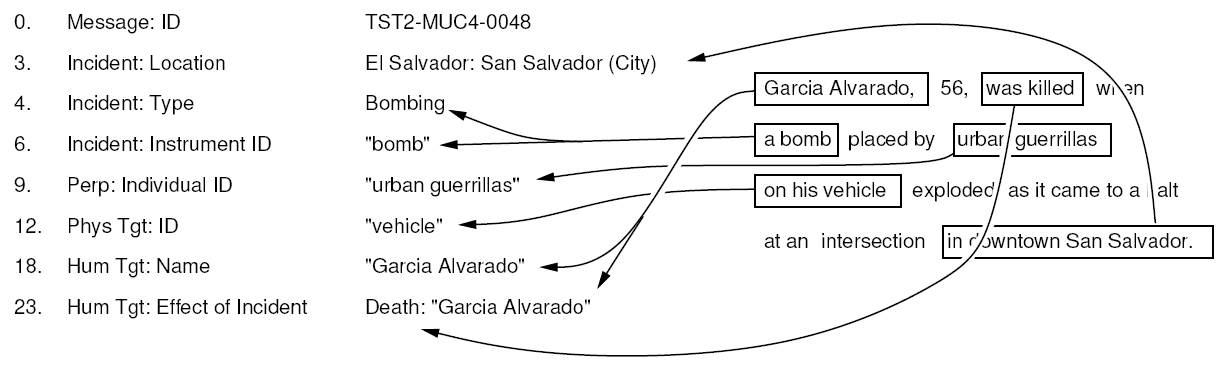
\includegraphics[width=\linewidth,keepaspectratio]{chunk-muc}
\end{center}
\end{frame}


%%%%%%%%%%%%%%%%%%%%%%%%%%%%%%%%%%%%%%%%%%%%%%%%%%%%%%%%%%%%%%%%%%%%%%%%%%%%%%%%%%
\begin{frame}[fragile]
  \frametitle{Ignoring Information: Lexical Acquisition}

  \begin{itemize}
  \item studying syntactic patterns, e.g. finding verbs in a corpus, displaying possible arguments
  \item e.g. \texttt{gave}, in 100 files of the Penn Treebank corpus
  \item replaced internal details of each noun phrase with \texttt{NP}

\begin{lstlisting}
  gave NP
  gave up NP in NP
  gave NP up
  gave NP help
  gave NP to NP
\end{lstlisting}
    
  \item use in lexical acquisition, grammar development
  \end{itemize}
\end{frame}

%%%%%%%%%%%%%%%%%%%%%%%%%%%%%%%%%%%%%%%%%%%%%%%%%%%%%%%%%%%%%%%%%%%%%%%%%%%%%%%%%%
\begin{frame}[fragile]
  \frametitle{Analogy with Tokenization and Tagging}

  \begin{itemize}
  \item fundamental in NLP: segmentation and labelling
  \item tokenization and tagging \\[2ex]
	  \begin{center}
	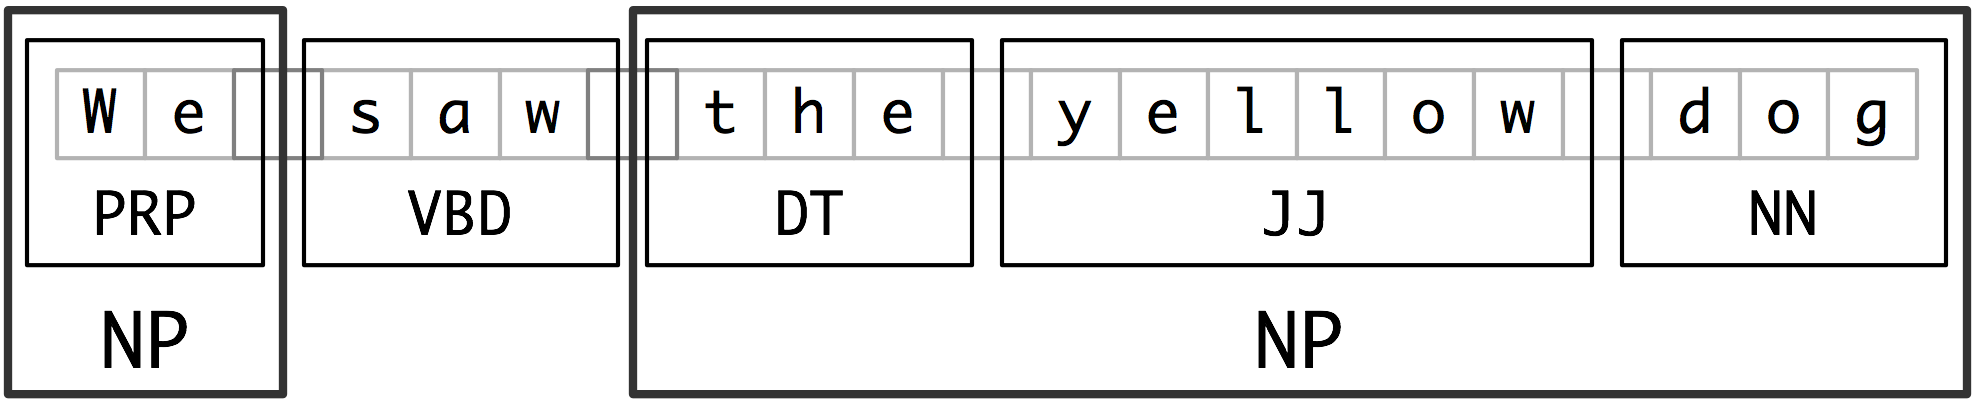
\includegraphics[width=\linewidth,keepaspectratio]{chunk-segmentation}
	\end{center}

  \item other similarities: skipping material; finite-state; application specific
  \end{itemize}
\end{frame}

%%%%%%%%%%%%%%%%%%%%%%%%%%%%%%%%%%%%%%%%%%%%%%%%%%%%%%%%%%%%%%%%%%%%%%%%%%%%%%%%%%
\begin{frame}[fragile]\frametitle{Chunking vs Parsing}
  \scriptsize

  \begin{itemize}
  \item Parsing
\begin{lstlisting}
  [
    [ G.K. Chesterton ],
    [
      [ author ] of
      [
        [ The Man ] who was
        [ Thursday ]
      ]
    ]
  ]
\end{lstlisting}

  \item Chunking:
\begin{lstlisting}
  [ G.K. Chesterton ],
  [ author ] of
  [ The Man ] who was
  [ Thursday ]
\end{lstlisting}
\end{itemize}
\end{frame}

%%%%%%%%%%%%%%%%%%%%%%%%%%%%%%%%%%%%%%%%%%%%%%%%%%%%%%%%%%%%%%%%%%%%%%%%%%%%%%%%%%
\begin{frame}[fragile]\frametitle{Chunking vs Parsing}
  \begin{itemize}
  \item flat vs nested
  \item context
  \item robustness
  \item efficiency
  \item methodology
  \end{itemize}
\end{frame}

%%%%%%%%%%%%%%%%%%%%%%%%%%%%%%%%%%%%%%%%%%%%%%%%%%%%%%%%%%%%%%%%%%%%%%%%%%%%%%%%%%
\begin{frame}[fragile]\frametitle{Perfection is unattainable}
\begin{lstlisting}
  1. Prepositional phrase:
  [
    [ I ]
    [ turned ]
    [ off the spectroroute ]
  ]

  2. Verb-particle construction:
  [
    [ I ]
    [ turned off ]
    [ the spectroroute ]
  ]
\end{lstlisting}
\end{frame}

%%%%%%%%%%%%%%%%%%%%%%%%%%%%%%%%%%%%%%%%%%%%%%%%%%%%%%%%%%
\begin{frame}[fragile]
  \frametitle{Tag Representation}
\begin{center}
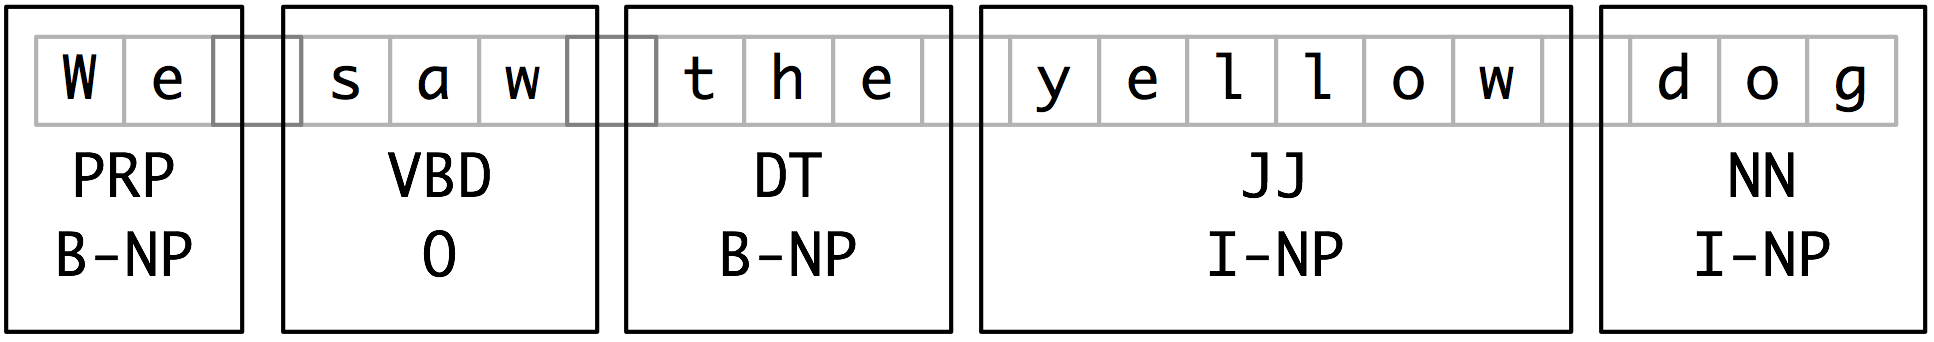
\includegraphics[width=\linewidth,keepaspectratio]{chunk-tagrep}
\end{center}
\end{frame}


%%%%%%%%%%%%%%%%%%%%%%%%%%%%%%%%%%%%%%%%%%%%%%%%%%%%%%%%%%
\begin{frame}[fragile]
  \frametitle{Tree Representation}
\begin{center}
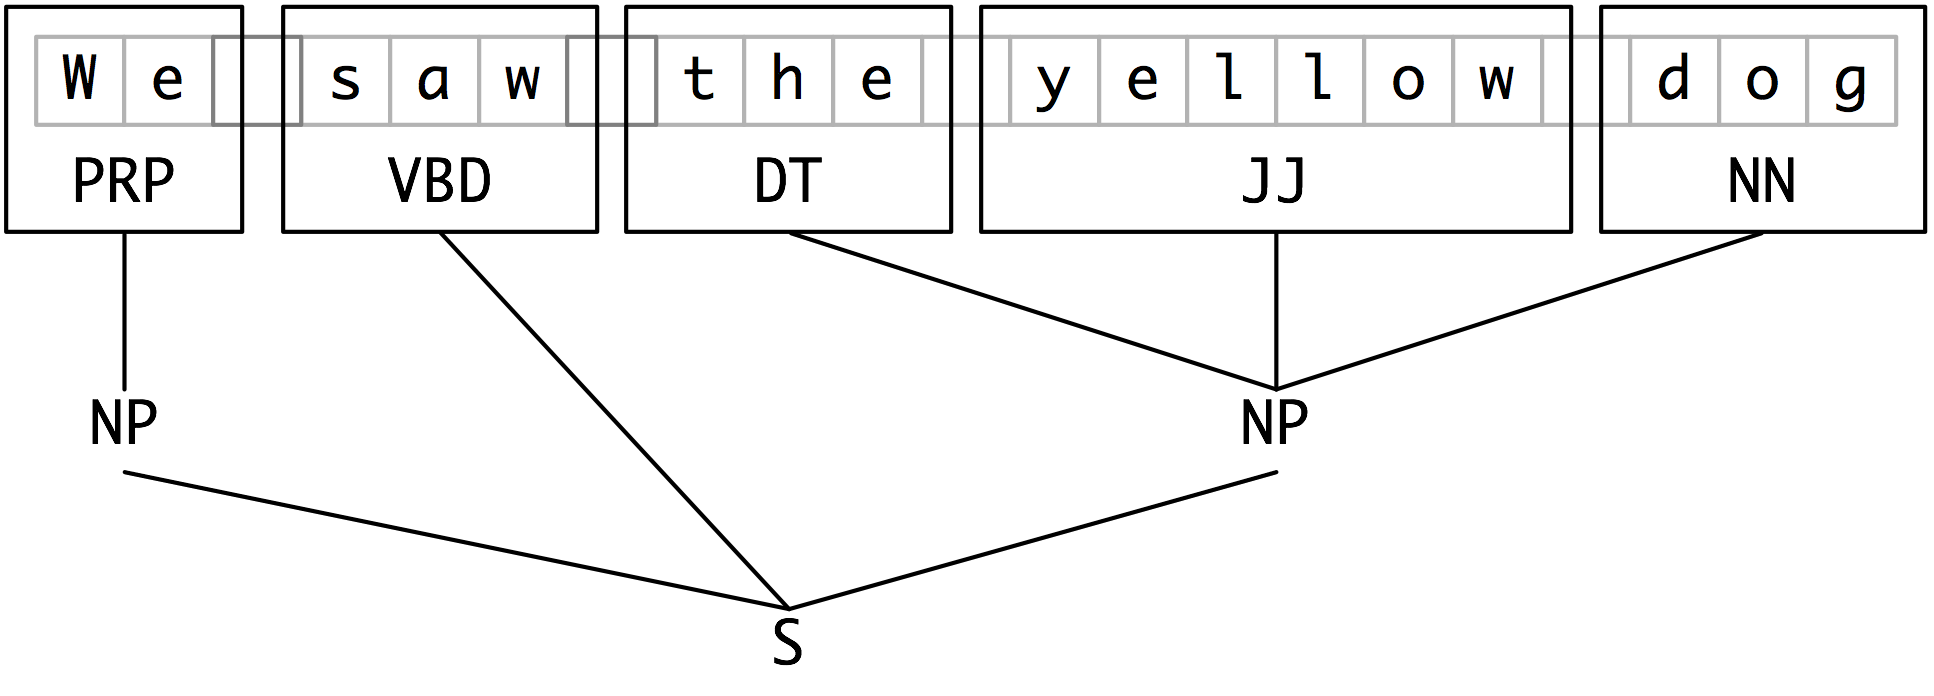
\includegraphics[width=\linewidth,keepaspectratio]{chunk-treerep}
\end{center}
\end{frame}

%%%%%%%%%%%%%%%%%%%%%%%%%%%%%%%%%%%%%%%%%%%%%%%%%%%%%%%%%%%%%%%%%%%%%%%%%%%%%%%%%%
\begin{frame}[fragile]\frametitle{Chunk Structures}
\begin{lstlisting}
  (S: (NP: 'I')
      'saw'
      (NP: 'the' 'big' 'dog')
      'on'
      (NP: 'the' 'hill'))
\end{lstlisting}
  \begin{itemize}
  \item Demonstration: reading chunk structures from Treebank and CoNLL-2000 corpora
  \end{itemize}
\end{frame}

%%%%%%%%%%%%%%%%%%%%%%%%%%%%%%%%%%%%%%%%%%%%%%%%%%%%%%%%%%%%%%%%%%%%%%%%%%%%%%%%%%
\begin{frame}[fragile] \frametitle{Chunk Parsing}
  \small

  \begin{itemize}
  \item regular expressions over part-of-speech tags: \texttt{parse.RegexpChunk}
  \item \textit{Tag string:} a string consisting of tags
    delimited with angle-brackets,
    e.g. \verb/<DT><JJ><NN><VBD><DT><NN>/
  \item \textit{Tag pattern:} regular expression over tag strings
    \begin{itemize}
    \item \verb/<DT><JJ>?<NN>/
    \item \verb/<NN|JJ>+/
    \item \verb/<NN.*>/
    \end{itemize}
  \item chunk a sequence of words matching a tag pattern: \texttt{parse.ChunkRule}

\begin{lstlisting}
    >>> grammar = ''NP: {<DT|NN>+}  # Chunk sequences of DT and NN'''
\end{lstlisting}

  \end{itemize}
\end{frame}

%%%%%%%%%%%%%%%%%%%%%%%%%%%%%%%%%%%%%%%%%%%%%%%%%%%%%%%%%%%%%%%%%%%%%%%%%%%%%%%%%%
\begin{frame}[fragile]\frametitle{Evaluating Chunk Parsers}

  \begin{itemize}
  \item Process:
    \begin{itemize}
    \item take some already chunked text
    \item strip off the chunks
    \item rechunk it
    \item compare the result with the original chunked text
    \end{itemize}
  \item \texttt{ChunkScore.score()}
    \begin{itemize}
    \item \textit{precision}: what fraction of the returned chunks were correct?
    \item \textit{recall}: what fraction of correct chunks were returned?
    \end{itemize}
  \end{itemize}
\end{frame}


%%%%%%%%%%%%%%%%%%%%%%%%%%%%%%%%%%%%%%%%%%%%%%%%%%%%%%%%%%
\begin{frame}[fragile]\frametitle{Precision and Recall}
\begin{center}
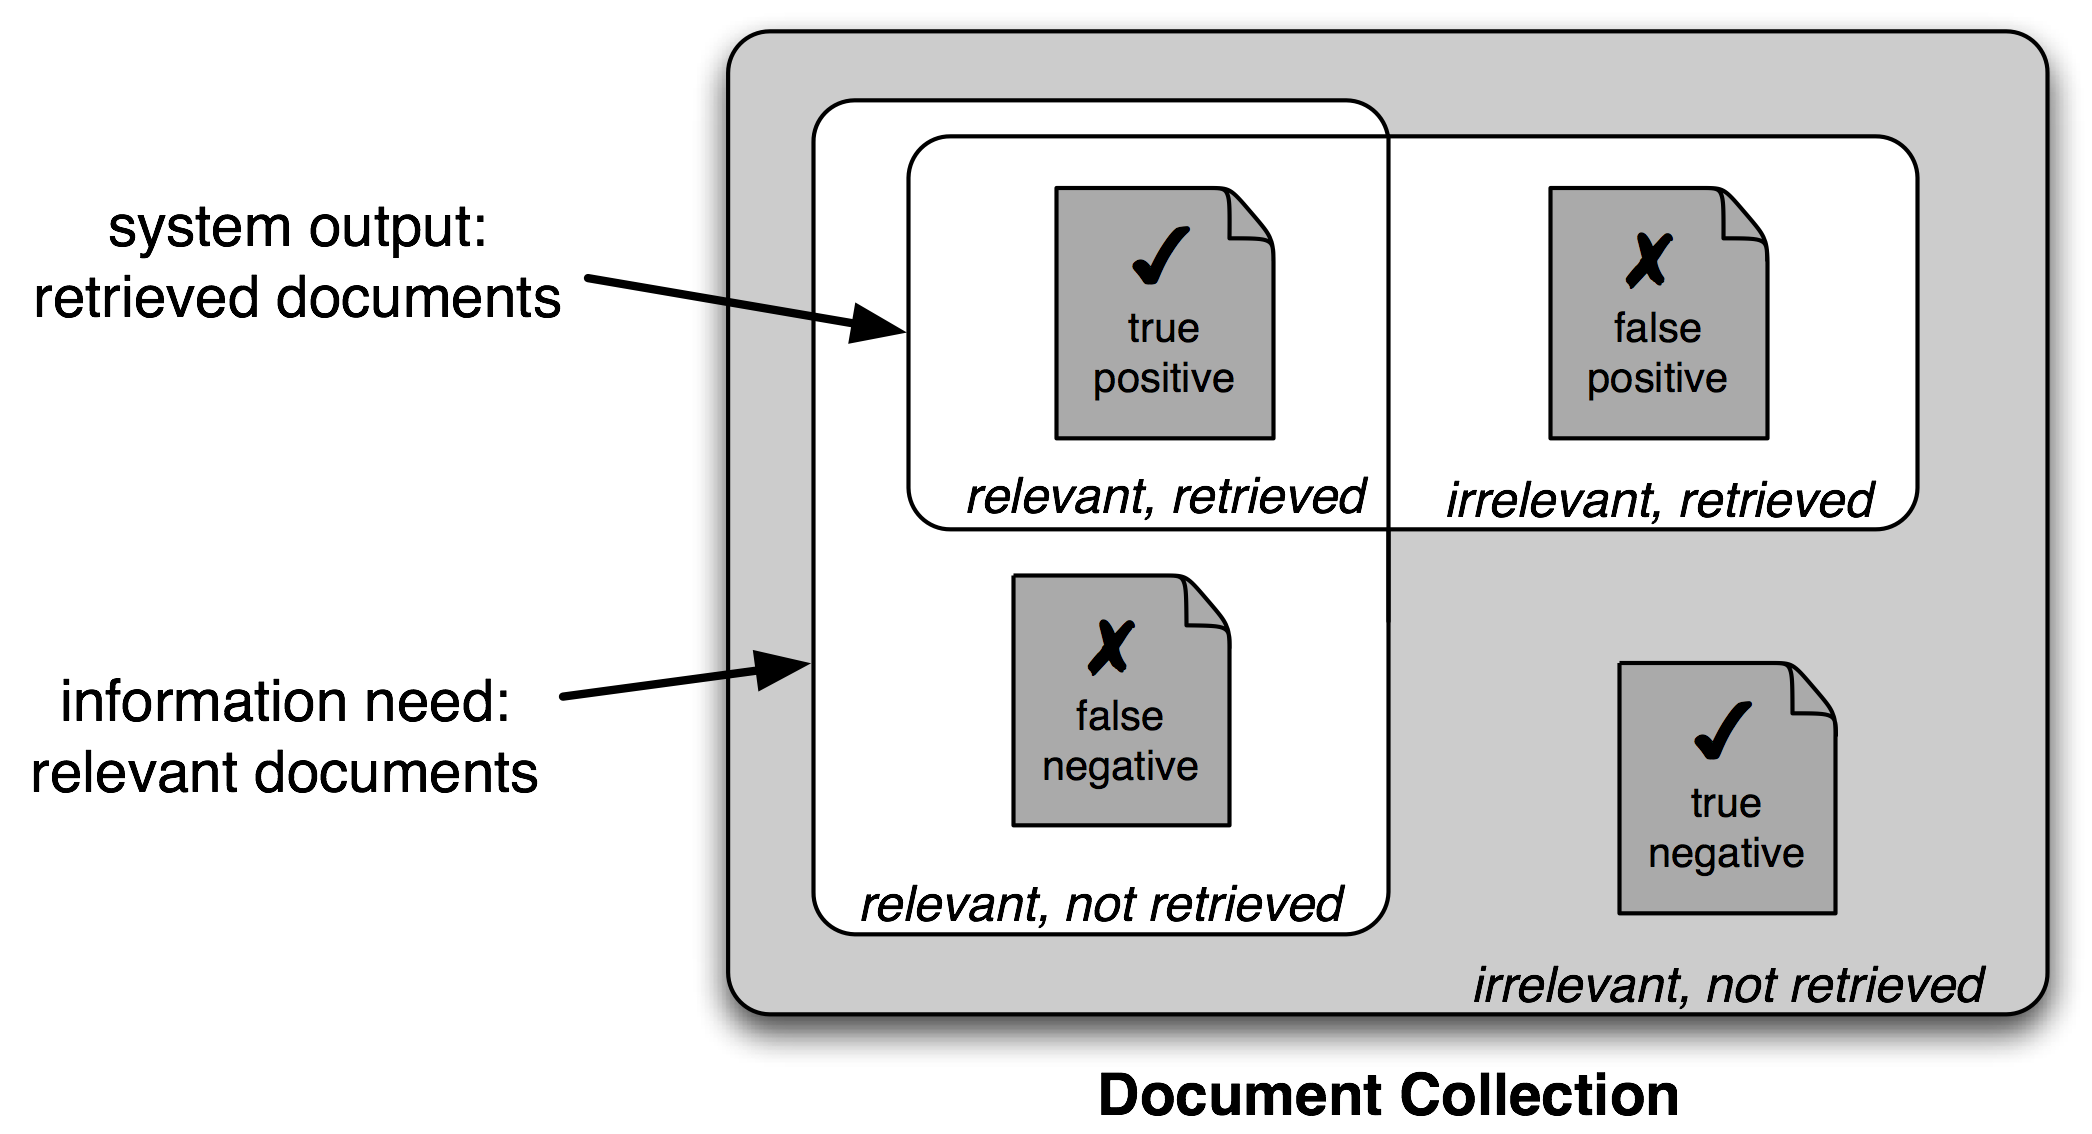
\includegraphics[width=\linewidth,keepaspectratio]{precision-recall}
\end{center}
\end{frame}

%%%%%%%%%%%%%%%%%%%%%%%%%%%%%%%%%%%%%%%%%%%%%%%%%%%%%%%%%%%%%%%%%%%%%%%%%%%%%%%%%%
\begin{frame}[fragile]\frametitle{Evaluation Methodology}
  \begin{itemize}
  \item Baseline:
    \begin{itemize}
    \item How hard is chunking?
    \item What is a good baseline for evaluation?
    \end{itemize}
  \item Bake-off
  \end{itemize}
\end{frame}

%%%%%%%%%%%%%%%%%%%%%%%%%%%%%%%%%%%%%%%%%%%%%%%%%%%%%%%%%%%%%%%%%%%%%%%%%%%%%%%%%%
\begin{frame}[fragile]\frametitle{Development Methodology}
  \begin{itemize}
  \item approaches
    \begin{itemize}
    \item different rules and combinations
    \item hand-crafted vs automatic
    \end{itemize}
  \item focus on diagnosis:
    \begin{itemize}
    \item manual
    \item utility functions
    \item error analysis
    \item evaluation
    \end{itemize}
  \end{itemize}
\end{frame}

%%%%%%%%%%%%%%%%%%%%%%%%%%%%%%%%%%%%%%%%%%%%%%%%%%%%%%%%%%%%%%%%%%%%%%%%%%%%%%%%%%
\begin{frame}[fragile]\frametitle{Conclusion}
  \begin{itemize}
  \item light-weight methods: as seen in tagging
  \item applications: extraction, lexical acquisition\\
    (aside: chunking as a utility method in parsing)
  \item next: parsing
  \item but first: switch to application focus
  \end{itemize}
\end{frame}


